% 曲面积分 通量

\pentry{矢量场\upref{Vfield}, 二重积分\upref{IntN}}
% 未完成: 预备:曲面的法向量

我们先来看一个例子

\begin{exam}{匀速水流场的流量}

\begin{figure}[ht]
\centering
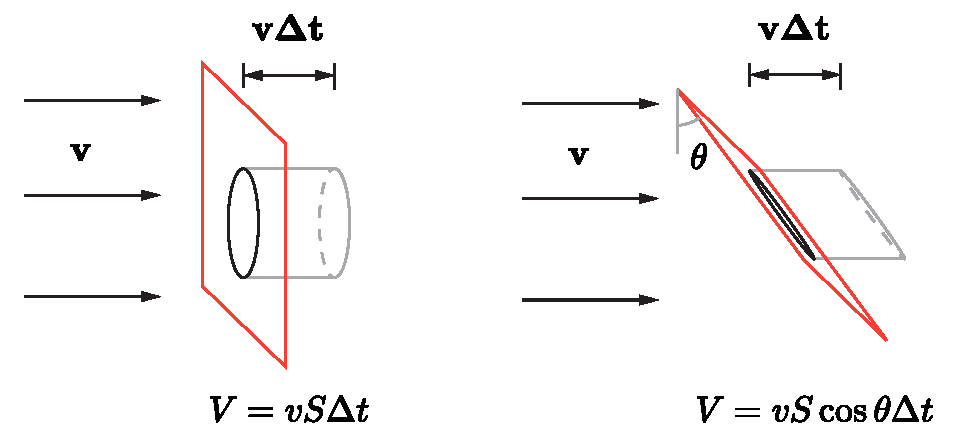
\includegraphics[width=10.5cm]{./figures/SurInt1.pdf}
\caption{匀速水流场的流量} \label{SurInt_fig1}
\end{figure}

水流中各点的速度可以看做一个矢量场 $\vec v(\vec r)$, 假设 $\vec v(\vec r) = \vec v_0$ 是一个常矢量. 在矢量场中取一个平面, 平面的法向量与 $\vec v_0$ 的夹角为 $\theta$, 在平面上选一个面积为 $S$ 的区域, 求单位时间通过该区域的水流的体积.

先来考虑 $\theta = 0$ 的情况, 在 $\Delta t$ 时间内, 流过区域的水是一个柱体, 其底面积为 $S$, 高为 $v_0\Delta t$, 所以体积为 $v_0 S\Delta t$, 所以单位时间的体积等于流速乘以面积 $v_0 S$.

我们再来考虑 $\theta \ne 0$ 的情况, $\Delta t$ 时间内流过区域的水是一个斜柱体, 由图\autoref{SurInt_fig1} 可知其体积等于横截面积 $S\cos\theta$ 乘以斜边长度 $v_0\Delta t$ 即 $V = v_0 S\cos\theta\Delta t$, 所以单位时间流过的体积为 $v_0 S\cos\theta$. 可见随着 $\theta$ 增大, 流量变小, 直到 $\theta = \pi/2$ 时流量为 $0$.

现在试想速度场 $\vec v(\vec r)$ 不是常矢量, 且有限的平面改为有限的曲面, 要计算单位时间流过曲面的体积, 我们可以先将曲面划分成无穷多个小曲面, 每个曲面上的流速看做常矢量, 再按照上述的办法计算并求和即可.
\end{exam}

现在我们来定义一个矢量场在一个曲面上的\bb{曲面积分}\footnote{简称\bb{面积分}, 这时需要通过语境与 “二重积分\upref{IntN}” 区分开.}(或\bb{通量}). 假设矢量场与曲面都处处光滑, 令矢量场为 $\vec F(\vec r)$, 给曲面定义一个正方向, 并将曲面划分为许多面积为 $\Delta S_i$ 的小面元, 令其法向量为 $\uvec n_i$(与曲面正方向同侧), 则一块面元可以表示为 $\Delta \vec S_i = \Delta S_i \uvec n_i$. 当面元很小时可以假设其内部的矢量场为常矢量 $\vec F(\vec r_i)$, 则面积分被定义为
\begin{equation}\label{SurInt_eq1}
\int \vec F(\vec r) \vdot \dd{\vec S} = \lim_{\Delta S_i\to 0} \sum_i \vec F(\vec r_i) \vdot \Delta \vec S_i
\end{equation}

\subsection{直角坐标系中的曲面积分}
% 引用曲面的法向量
直角坐标系中的曲面可以表示为 $f(x,y,z) = 0$ 其法向量 $\uvec n(x,y,z)$ 等于 $\pm\grad f(x,y,z)$ 归一化. 令矢量场为 $\vec F(x,y,z)$, 应如何具体计算曲面积分呢? 

以下我们来讨论曲面可以表示为 $z = g(x,y)$ 的情况\footnote{如果不能表示为 $z = g(x,y)$, 但可以表示为 $x = g(y,z)$ 或 $y = g(x,z)$, 以下过程也类似.}. 将曲面沿 $x,y$ 方向划分成许多面元, 使每个面元在 $x,y$ 平面上的投影都是一个小长方形, 面积为 $\Delta x_i, \Delta y_j$, 面元上任意一点的坐标为 $[x_i, y_j, g(x_i,y_j)]$. 面元面积与投影面积的关系为 $\Delta S_{ij} \cos\theta = \Delta x_i \Delta y_j$, 其中 $\theta$ 是面元的法向量与 $z$ 轴的夹角, 所以 $\cos\theta = \uvec n\uvec z = n_z$. 所以, 矢量场在每个面元上的通量为
\begin{equation}
\vec F(\vec r_{ij}) \vdot \Delta \vec S_{ij} = \qty(\frac{n_x}{n_z}F_x + \frac{n_y}{n_z}F_y + F_z) \Delta x_i \Delta y_j
\end{equation}
其中 $\uvec n, \vec F$ 的个分量在 $[x_i, y_j, g(x_i,y_j)]$ 处取值.

由\autoref{SurInt_eq1} 的定义, 曲面积分为
\begin{equation}\label{SurInt_eq3}
\ali{
\int \vec F(\vec r) \vdot \dd{\vec S} &= \lim_{\substack{\Delta x_i\to 0\\ \Delta y_i\to 0}} \sum_{ij} \vec F(\vec r_{ij}) \vdot \Delta \vec S_{ij}\\
& = \iint \frac{n_x}{n_z}F_x \dd{x}\dd{y} + \iint \frac{n_y}{n_z}F_y \dd{x}\dd{y} + \iint F_z \dd{x}\dd{y}
}\end{equation}
这样, 我们就把曲面积分转换成了三个二重积分. 这三个二重积分分别等于矢量场的三个分量对曲面通量的贡献. 特殊地, 若曲面方程可以记为 $z = g_1(x,y), x = g_2(y,z), y = g_3(x,z)$ 中的任意一种形式, 我们也可以将曲面积分记为
\begin{equation}
\int \vec F(\vec r) \vdot \dd{\vec S} = \iint F_x \dd{y}\dd{z} + \iint F_y \dd{x}\dd{z} + \iint F_z \dd{x}\dd{y}
\end{equation}

\begin{exam}{}
求场 $\vec F(\vec r) = \vec r$ 在曲面(正方向向上) $z = x^2 + y^2 \quad (x, y\in [-1,1])$ 上的通量.

我们先求曲面的法向量, 令 $f(x,y,z) = x^2 + y^2 - z$, 则法向量的方向为 $\grad f = (2x, 2y, -1)$ 由于曲面的正方向向上, 我们将 $\grad f$ 取相反数然后归一化得到法向量
\begin{equation}
\uvec n = \frac{-2x}{\sqrt{4x^2 + 4y^2 + 1}}\uvec x + \frac{-2y}{\sqrt{4x^2 + 4y^2 + 1}}\uvec y + \frac{1}{\sqrt{4x^2 + 4y^2 + 1}}\uvec z
\end{equation}
将上式和 $\vec F(\vec r) = x\uvec x + y\uvec y + z\uvec z$ 代入\autoref{SurInt_eq3} 得
\begin{equation}
\ali{
\int \vec F(\vec r) \vdot \dd{\vec S} &= 
-\iint 2x^2 \dd{x}\dd{y} - \iint 2y^2 \dd{x}\dd{y} + \iint (x^2 + y^2) \dd{x}\dd{y}\\
&= -\eval{\frac43 x^3}_{-1}^1 -\eval{\frac43 y^3}_{-1}^1 + \eval{\frac23 x^3}_{-1}^1 + \eval{\frac23 y^3}_{-1}^1 = -\frac83
}\end{equation}

\end{exam}
